% --- EVALUATION AND RESULTS ---

\noindent This chapter presents the experimental results across four task scales, comparing all three algorithms.

\section{Overall and Severity-Specific Outage Analysis}

Table~\ref{tab:overall_outage} presents the overall outage probability averaged over 10 iterations per scenario.

\begin{table}[htbp]
\centering
\begin{tabular}{|c|c|c|c|}
\hline
\textbf{Scale} & \textbf{Greedy Placement} & \textbf{Baseline (M-DAFTO)} & \textbf{Proposed System} \\
\hline
250  & 0.00\% & 0.92\% & \textbf{0.16\%} \\
500  & 0.00\% & 1.34\% & \textbf{0.02\%} \\
1000 & 0.00\% & 3.65\% & \textbf{0.02\%} \\
2000 & 13.15\% & 20.46\% & \textbf{13.15\%} \\
\hline
\end{tabular}
\caption{Overall outage probability (\%) across four task scales.}
\label{tab:overall_outage}
\end{table}

Under normal-to-high load (250--1000 tasks), the proposed method reduces overall outage dramatically: from 0.92\% to 0.16\% at 250 tasks, from 1.34\% to 0.02\% at 500 tasks, and from 3.65\% to 0.02\% at 1000 tasks. Under extreme overload (2000 tasks), the proposed method matches GPM at 13.15\%, significantly better than the baseline's 20.46\%.

Table~\ref{tab:major_outage} shows the Major task (critical operations) outage --- the most important safety metric.

\begin{table}[htbp]
\centering
\begin{tabular}{|c|c|c|c|}
\hline
\textbf{Scale} & \textbf{Greedy Placement} & \textbf{Baseline (M-DAFTO)} & \textbf{Proposed System} \\
\hline
250  & 0.00\% & 1.06\% & \textbf{0.00\%} \\
500  & 0.00\% & 1.32\% & \textbf{0.00\%} \\
1000 & 0.00\% & 3.72\% & \textbf{0.00\%} \\
2000 & 13.02\% & 20.46\% & \textbf{9.36\%} \\
\hline
\end{tabular}
\caption{Major task outage probability (\%) across four task scales.}
\label{tab:major_outage}
\end{table}

The most important result is that under normal load (250--1000 tasks), the proposed algorithm achieves \textbf{0\% Major outage} --- zero critical surgeries fail to get assigned. The baseline has 1--4\% Major outage at the same scales. Under extreme overload (2000 tasks), Major outage drops from 20.46\% to 9.36\%, a 54.3\% reduction even when the system is saturated.

\begin{figure}[htbp]
\centering
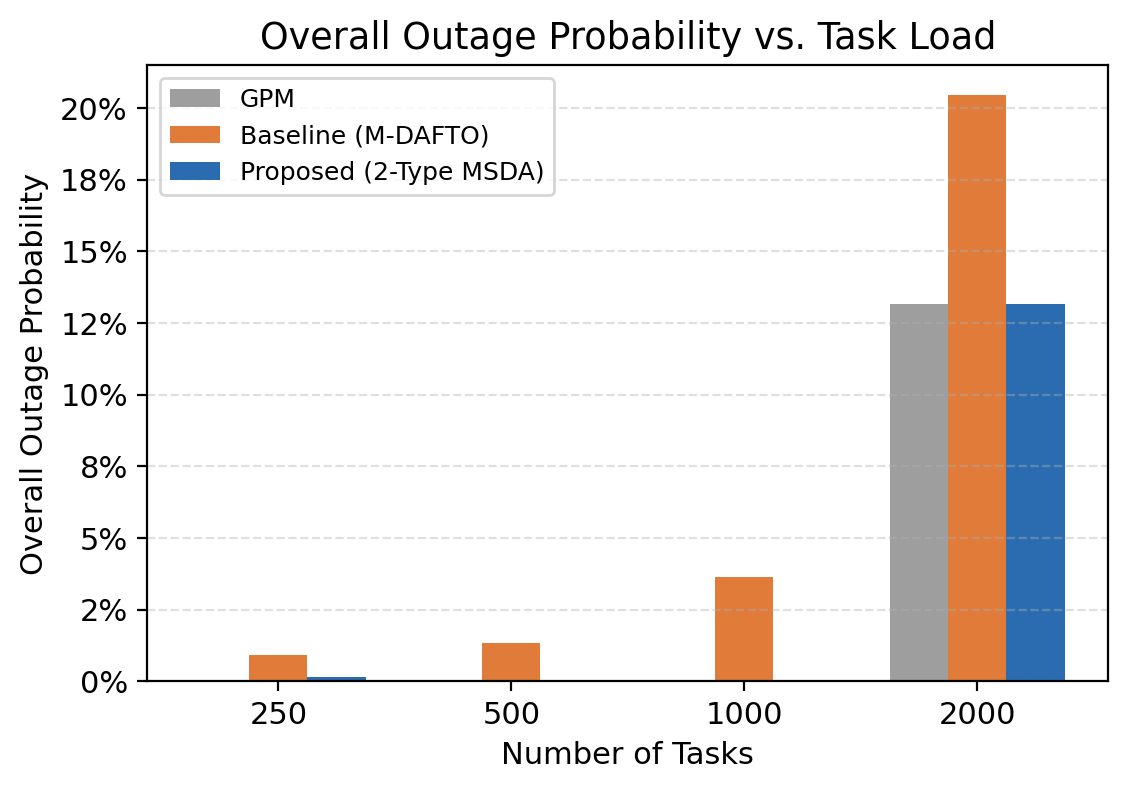
\includegraphics[width=0.75\textwidth]{Images/fig_overall_outage.png}
\caption{Overall outage probability comparison across four task scales.}
\label{fig:overall_outage}
\end{figure}

\begin{figure}[htbp]
\centering
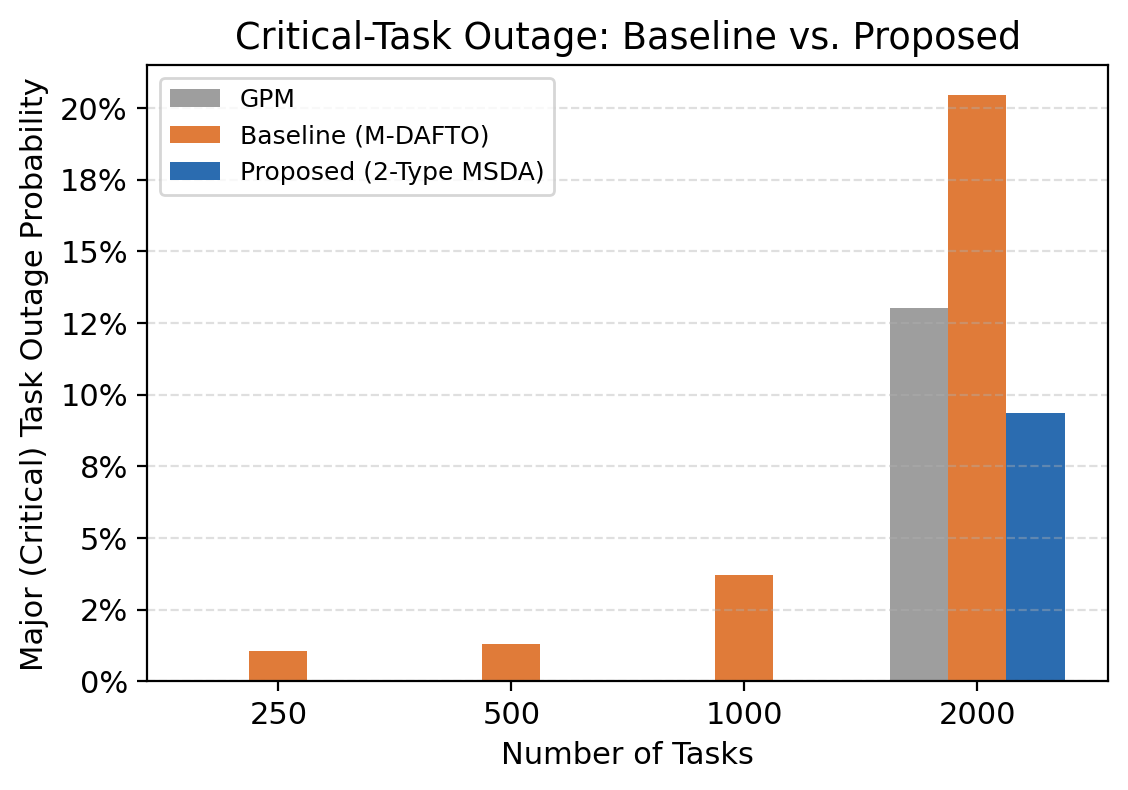
\includegraphics[width=0.75\textwidth]{Images/fig_major_outage.png}
\caption{Major task outage probability comparison across four task scales.}
\label{fig:major_outage}
\end{figure}

Table~\ref{tab:outage_reduction} summarises the outage reduction achieved by the proposed method relative to the baseline.

\begin{table}[htbp]
\centering
\begin{tabular}{|c|c|c|}
\hline
\textbf{Scale} & \textbf{Overall Outage Reduction} & \textbf{Major Outage Reduction} \\
\hline
250  & 82.6\% & $\sim$100\% \\
500  & 98.5\% & $\sim$100\% \\
1000 & 99.5\% & $\sim$100\% \\
2000 & 35.7\% & 54.3\% \\
\hline
\textbf{Average} & \textbf{$\sim$79\%} & \textbf{$\sim$89\%} \\
\hline
\end{tabular}
\caption{Outage reduction of the proposed method relative to the baseline M-DAFTO.}
\label{tab:outage_reduction}
\end{table}

The S-4 scenario (2000 tasks) represents extreme overload where total task demand exceeds the combined capacity of all fog nodes. Even in this saturated case, the proposed method still reduces Major outage by 54.3\%. The reduction is smaller than at lower scales because there are simply not enough fog node slots for all tasks, regardless of the matching algorithm used.

\section{Delay, Energy, and Satisfaction Trade-offs}

\subsection{Delay and Energy Comparison}

\begin{table}[htbp]
\centering
\begin{tabular}{|c|c|c|c|c|c|c|}
\hline
\textbf{Scale} & \multicolumn{2}{c|}{\textbf{Greedy Placement}} & \multicolumn{2}{c|}{\textbf{Baseline}} & \multicolumn{2}{c|}{\textbf{Proposed}} \\
\cline{2-7}
 & \textbf{AvgDelay} & \textbf{Energy} & \textbf{AvgDelay} & \textbf{Energy} & \textbf{AvgDelay} & \textbf{Energy} \\
\hline
250  & 20.66 & 5142.81 & 12.65 & 3102.92 & 12.87 & 3189.85 \\
500  & 20.43 & 10168.93 & 12.67 & 6186.92 & 12.83 & 6366.47 \\
1000 & 18.07 & 17976.69 & 13.36 & 12739.14 & 13.70 & 13604.51 \\
2000 & 16.17 & 28033.18 & 14.53 & 22967.31 & 16.22 & 28110.36 \\
\hline
\end{tabular}
\caption{Average delay (seconds) and total energy (Joules) across all algorithms.}
\label{tab:delay_energy}
\end{table}

The proposed method has slightly higher average delay than the baseline (e.g., 12.87 vs 12.65 at 250 tasks). This is because the 2-Type MSDA sacrifices delay-optimal placement to ensure Major tasks are assigned to fog nodes that satisfy the severity-aware quota constraints. In healthcare, this is an acceptable trade-off: a minor increase in processing delay is far preferable to a critical surgery going unassigned.

\subsection{Task and FN Satisfaction}

\begin{table}[htbp]
\centering
\begin{tabular}{|c|c|c|c|}
\hline
\textbf{Scale} & \textbf{Greedy Placement} & \textbf{Baseline (M-DAFTO)} & \textbf{Proposed System} \\
\hline
250  & 9.04\% & 71.14\% & 69.96\% \\
500  & 14.09\% & 68.26\% & 67.46\% \\
1000 & 21.72\% & 60.62\% & 59.31\% \\
2000 & 33.77\% & 40.27\% & 32.83\% \\
\hline
\end{tabular}
\caption{Task satisfaction (\%) across four task scales.}
\label{tab:task_satisfaction}
\end{table}

Task satisfaction is slightly lower for the proposed method (e.g., 69.96\% vs 71.14\% at 250 tasks) because the severity-aware matching sometimes assigns tasks to their second or third preferred fog node to ensure Major quotas are met. However, the difference is small (within 2 percentage points at most scales).

\begin{table}[htbp]
\centering
\begin{tabular}{|c|c|c|c|}
\hline
\textbf{Scale} & \textbf{Greedy Placement} & \textbf{Baseline (M-DAFTO)} & \textbf{Proposed System} \\
\hline
250  & 10.04\% & 10.54\% & 10.34\% \\
500  & 12.05\% & 19.50\% & 18.85\% \\
1000 & 25.00\% & 34.57\% & 35.25\% \\
2000 & 50.43\% & 50.22\% & \textbf{59.08\%} \\
\hline
\end{tabular}
\caption{FN satisfaction (\%) across four task scales.}
\label{tab:fn_satisfaction}
\end{table}

\begin{figure}[htbp]
\centering
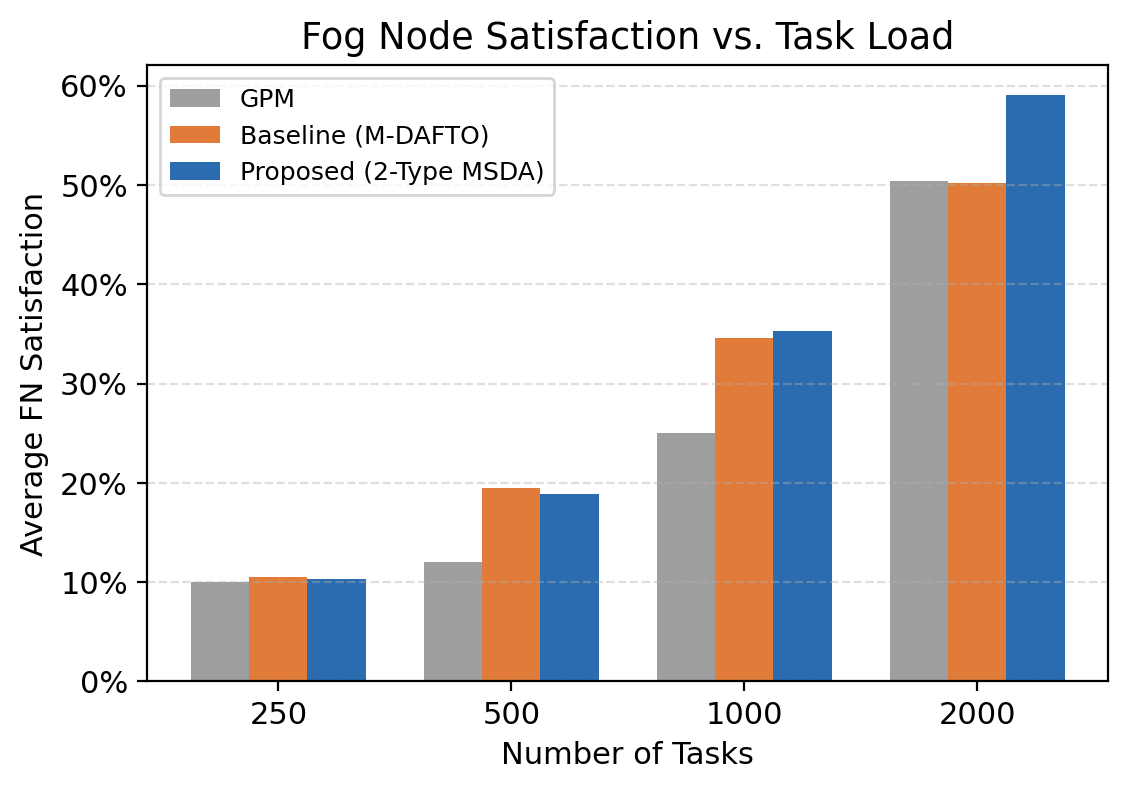
\includegraphics[width=0.75\textwidth]{Images/fig_fn_satisfaction.png}
\caption{FN satisfaction comparison across four task scales.}
\label{fig:fn_satisfaction}
\end{figure}

FN satisfaction improves under overload (59.08\% vs 50.22\% at 2000 tasks), showing that the 2-Type system distributes tasks more effectively by leveraging separate Major/Minor quota tracking.

\subsection{GPM Comparison}

GPM shows 0\% outage at 250--1000 tasks because it simply fills fog nodes greedily by capacity. However, its task satisfaction is extremely low (9--34\%) because it ignores preferences entirely. GPM fails at 2000 tasks (13.15\% outage) because it has no quota-based fairness mechanism. This confirms that greedy approaches, while simple, are unsuitable for healthcare IoT where both task satisfaction and critical-task protection matter.